\selectlanguage{ngerman}%
\frenchspacing%
\begin{ledgroupsized}[r]{120mm}%
\footnotesize%
\pstart%
\noindent%
\textbf{Überlieferung:}%
\pend%
\end{ledgroupsized}%
\begin{ledgroupsized}[r]{114mm}%
\footnotesize%
\pstart%
\parindent -6mm%
\makebox[6mm][l]{\textit{L}}%
Aufzeichnung:
LH XXXV 14,\;2 Bl.\;4.
Ein Blatt 4\textsuperscript{o},
Ränder zum Teil beschnitten;
römisches Papier (ohne Wasserzeichen). 
Eine volle Seite auf Bl.\;\href{\Scan{LH_35_14_02_004r}}{4\,r\textsuperscript{o}}
und vier Zeilen auf Bl.\;\href{\Scan{LH_35_14_02_004v}}{4\,v\textsuperscript{o}};
der Rest ist unbeschrieben.
\pend%
\end{ledgroupsized}%
\vspace{5mm}%
\begin{ledgroup}%
\footnotesize%
\pstart%
\noindent%
\textbf{Datierungsgründe:}
Die Datierung der Aufzeichnung N.\;\ref{58218} beruht auf Eigenschaften des Textträgers.
Siehe die ausführliche Begründung auf S.\;\pageref{58218_dat}.%
\pend%
\end{ledgroup}%
\selectlanguage{latin}%
\frenchspacing%
\vspace{8mm}%
\normalsize%
\pstart%
\noindent%
\lbrack%
\href{\Scan{LH_35_14_02_004r}}%
{4\,r\textsuperscript{o}}%
\rbrack\
Ut examinetur
quomodo parte liquidi mota%
\indexS{liquidum}
moveatur totum,%
\indexS{motus liquidi}
consideranda est ejus tenacitas.%
\indexS{tenacitas liquidi}
Videndum est ergo
quomodo corpus unum moveat aliud%
\indexS{corpus movens aliud ope filorum}
ope filorum%
\indexS{filum tendibile}
\edtext{%
tendibilium,
ut si trahat ope fili%
}{%
\lemma{tendibilium,}%
\Bfootnote{%
\textit{(1)}~seu ope asperi %
\textit{(2)}~ut si trahat ope fili%
~\textit{L}%
}}
quod tendi potest%
\indexS{filum tendibile}
et tandem nimis tensum rumpitur,%
\indexS{filum tensum}%
\indexS{filum ruptum}
ita ut tunc non sequantur se amplius%
\lbrack;\rbrack\
\edtext{%
vel sine filo,%
\indexS{filum tendibile}%
}{%
\lemma{vel}%
\Bfootnote{%
\textit{(1)}~si non r %
\textit{(2)}~sine filo,%
~\textit{L}%
}}
ope ansae curvae%
\indexS{ansa curva}
quae flectit sese%
\indexS{ansa flectens se}
ob elastrum%
\indexS{elastrum ansae}
et denique trahentem deserit.
Vel dum unum corpus alterum radit%
\indexS{corpus radens alterum}
et asperitates ejus elasticas vincit,%
\indexS{asperitas elastica}
et partim corpus alterum secum%
\indexS{corpus secum abripens alterum}
\edtext{%
abripit,
partim quatenus%
}{%
\lemma{abripit, partim}%
\Bfootnote{%
\bars{in \textit{streicht Hrsg.}} quatenus %
~\textit{L}%
}}
elastra asperitatum%
\indexS{elastrum asperitatis}
cedunt%
\indexS{elastrum cedens}
deserit.
Sit ergo corpus \textit{A} in motu%
\indexS{corpus in motu}%
\indexS{motus corporis}
et corpus \textit{B} radat,%
\indexS{corpus radens alterum}
et occurrant sibi eorum asperitates%
\indexS{asperitas elastica}
\textit{m} et \textit{n}.
Quaeritur
quantum motus accipiat \textit{B},
et quantum virium accipiat%
\indexS{vis accepta ab elastro}
elaster%
\indexS{elaster accipiens vim}%
\indexS{elaster asperitatis}
\edtext{%
\textit{mn}.
Idem%
}{%
\lemma{\textit{mn}}%
\Bfootnote{%
\textit{(1)}~, an %
\textit{(2)}~. Idem%
~\textit{L}%
}}
est si \textit{A} in motum concitatum%
\indexS{corpus concitatum in motum}%
\indexS{motus corporis}
filum intendat%
\indexS{filum tensum}
et ejus ope%
\indexS{filum tendibile}
\edtext{%
trahat~\textit{B}.%
\indexS{corpus tractum ope filorum}
Utrobique
in quantum Elaterium resistit,%
\indexS{elaterium resistens motui}
in tantum facit%
}{%
\lemma{trahat~\textit{B}.}%
\Bfootnote{%
\textit{(1)}~Quamquam hic sit illud peculiare, quod Elastrum semper non tantum facit %
\textit{(2)}~Utrobique in %
\lbrack...\rbrack\ tantum facit%
~\textit{L}%
}}
motum%
\indexS{motus communicatus}%
\indexS{communicatio motus}
\edlabel{LH_35_14_02_004_004r_1a}%
communicari.%
\edtext{%
}{\xxref{LH_35_14_02_004_004r_1a}{LH_35_14_02_004_004r_1b}\lemma{communicari.}%
\Bfootnote{%
\lbrack/\rbrack\ %
\textit{(1)}~Ponamus primum aliquid potentiae dari Elastro, nam %
\lbrack/\rbrack\ %
\textit{(2)}~Initio elastrum %
\bars{\textit{mn} \textit{erg.}} potius tendetur, quia%
~\textit{L}%
}}
\pend%
\begin{edfigure}[2.25em][0em]
\hspace{-45mm}%
\includegraphics%
{gesamttex/edit_VIII-4/images/LH_35_14_02_004_d1_004r.pdf}
\edcaption%
{\hspace{-46mm}\lbrack \textit{Fig.\:1}\rbrack}%
\vspace{-5.5em}%
\hspace{45mm}%
\includegraphics%
{gesamttex/edit_VIII-4/images/LH_35_14_02_004_d2_004r.pdf}
\edcaption[0.5em]{\hspace{43mm}\lbrack\textit{Fig.\:2}\rbrack}%
\end{edfigure}%
\newpage%
\begin{edfigure}[0em][1.25em]
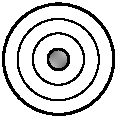
\includegraphics[width=0.15\textwidth]
{gesamttex/edit_VIII-4/images/LH_35_14_02_004_d3_004r.pdf}
\edcaption[0.5em]{\lbrack \textit{Fig.\:3}\rbrack}%
\end{edfigure}%
\pstart%
\noindent%
Initio elastrum \textit{mn} potius tendetur,%
\indexS{elastrum tensum}%
\indexS{elastrum resistens motui}
quia%
\edlabel{LH_35_14_02_004_004r_1b}
resistentia ejus%
\indexS{resistentia elastri ad tensionem}
ad tensionem quantulamcunque%
\indexS{tensio elastri quantulacunque}
nulla est.%
\indexS{tensio elastri nulla}
Sed aliquousque tensum%
\indexS{elastrum tensum}
resistet aliquantum,%
\indexS{elastrum resistens motui}
et adeo movebitur et aliquantum corpus \textit{B};
et quia
\edtext{%
causa%
\indexS{causa elastri tensi}
cur elastrum tendi cogatur,%
\indexS{elastrum coactum tendi}%
}{%
\lemma{causa}%
\Bfootnote{%
\textit{(1)}~cur resiste %
\textit{(2)}~cur elastrum tendi cogatur,%
~\textit{L}%
}}
est
quod motui
\edtext{%
resistit~\textit{B},
tantum semper movebitur \textit{B}%
}{%
\lemma{resistit \textit{B},}%
\Bfootnote{%
\textit{(1)}~ideo eousque semper mo %
\textit{(2)}~tantum semper movebitur \textit{B}%
~\textit{L}%
}}
ut non majore vi%
\indexS{vis tendens elastrum}
tendatur Elastrum%
\indexS{elastrum tensum}
quam opus est ad movendum~\textit{B}.
Cum igitur superato Elastro%
\indexS{elastrum superatum}
\edtext{%
\textit{mn}%
}{%
\lemma{\textit{mn}}%
\Bfootnote{%
\textit{erg.\;L}%
}}
cesset translatio motus%
\indexS{translatio motus}%
\indexS{motus translatus}%
\lbrack,\rbrack\
sequitur %
tantum virium conferri corpori \textit{B},%
\indexS{vis collata corpori ab elastro}
ut vis ejus sit aequalis Elastro tenso.%
\indexS{vis aequalis elastro tenso}%
\indexS{elastrum tensum}
Et proinde
\edtext{%
\lbrack vis\rbrack%
}{%
\lemma{celeritas}%
\Bfootnote{%
\textit{L\;ändert Hrsg.}%
}}
quae corpori \textit{B} affertur%
\indexS{celeritas allata corpori ab alio}
a corpore \textit{A}
est eadem,
sive magna sive parva sit velocitas%
\indexS{velocitas corporis tendentis elastrum}
ipsius \textit{A};
dimidium scilicet virium Elastri.%
\indexS{vis elastri}%
\indexS{elastrum tensum}
Et ideo
si multa simul Elastra tendantur,%
\indexS{elastra simul tensa}
seu superficies radens%
\indexS{superficies radens}
sit longa,
erit motus%
\indexS{motus acceptus}
quem accipit
\edtext{%
\lbrack\textit{B}\rbrack%
}{%
\lemma{\textit{A}}%
\Bfootnote{%
\textit{L\;ändert Hrsg.}%
}}
in ratione directa
\edtext{%
Elastricitatis,%
\indexS{elastricitas}
seu connexionis,
et reciproca%
}{%
\lemma{Elastricitatis\lbrack\textit{!}\rbrack}%
\Bfootnote{%
\textit{(1)}~et reciproca %
\textit{(2)}~, seu connexionis, et reciproca%
~\textit{L}%
}}
superficiei.%
\indexS{superficies radens}
Sed dum \textit{A} continuat motum %
(quod et intelligi potest
si \textit{A} esset cylindrus%
\indexS{cylinder convexus intra concavum}
\edtext{%
convexus%
}{%
\lemma{convexus}%
\Bfootnote{%
\textit{erg.\;L}%
}}
intra concavum cylindrum \textit{B}) %
repetitur impressio aliquousque.%
\indexS{impressio motus repetita}
Idque tamdiu,
donec motus fiat conspirans,%
\indexS{motus conspirans}
seu donec se mutuo non deserant.%
\indexS{corpora se mutuo non deserantia}
Verum si extrema quaedam sit superficies immota,%
\indexS{superficies immota}
tunc ipsa perinde resistit%
\indexS{superficies resistens motui}
ac si ipsa in contrariam partem moveretur%
\indexS{superficiens movens in partem contrariam}
quiescente incluso:%
\indexS{corpus quiescens}
itaque hoc
\edtext{%
casu non%
}{%
\lemma{casu}%
\Bfootnote{%
\bars{\textlangle vero\textrangle\ \textit{gestr.}} non%
~\textit{L}%
}}
potest unquam obtineri consensus,%
\indexS{consensus}
sed tandem continuatis resistentiis elasticis superandis%
\indexS{resistentia elastica}
necesse est absorberi motum.%
\indexS{motus absorptus}%
\indexS{absorptio motus}
Quod de sphaera%
\indexS{sphaera}
idem et de cylindro%
\indexS{cylinder}
et aliis figuris
quibuscunque assero%
\lbrack:\rbrack\
nam cum cessat motus absorptio,%
\indexS{absorptio motus}
remanente tenacitate%
\indexS{tenacitas remanens post motum absorptum}%
\indexS{tenacitas fluidi}
necesse est
omnia moveri ut unum solidum.%
\indexS{mota ut unum solidum}
\lbrack%
\href{\Scan{LH_35_14_02_004v}}%
{4\,v\textsuperscript{o}}%
\rbrack\
\pend%
\pstart%
An etiam sine
\edtext{%
tenacitate%
\indexS{tenacitas fluidi}%
\indexS{fluidum}%
\lbrack,\rbrack\
una fluidi pars%
}{%
\lemma{tenacitate}%
\Bfootnote{%
\textit{(1)}~unum fluidum %
\textit{(2)}~una fluidi pars%
~\textit{L}%
}}
aliam moveat%
\indexS{pars fluidi movens aliam sine tenacitate}
dispiciendum est.
Videtur scilicet
ex ipsa natura materiae%
\indexS{natura materiae}%
\indexS{materia}
omnes partes habere inter se unitatem,%
\indexS{partes materiae habentes unitatem}
ut communis sit earum motus%
\indexS{motus communis partium materiae}
nisi quid impediat,
et
\lbrack\textit{Text bricht ab.}\rbrack%
\pend%
\newpage%
\pstart%
\noindent%
\centering%
*     *     *
\pend%
\vspace{3.0em}%
\selectlanguage{german}%
\frenchspacing%
\footnotesize%
\pstart%
\noindent%
\textls{Ausführliche Datierungsgründe:}%
\pagelabel{58218_dat}
Der Träger der titellosen und undatierten Aufzeichnung N.\;\ref{58218}, die den dynamischen Zusammenhang der Teile eines Fluidums erörtert, weist zwar kein Wasserzeichen auf, wohl aber gleiche sichtbare Eigenschaften wie eine Papiersorte, die Leibniz während seines Aufenthalts in Rom\indexO{Rom} verwendete, unter anderem für die erste Fassung seiner \textit{Dynamica}.\cite{01354}
Auf gleichem Papier sind ebenfalls die in diesem Band veröffentlichten Aufzeichnungen N.\;\ref{58656-A}, N.\;\ref{58258} und N.\;\ref{58235} überliefert %
(siehe die ausführlichen Datierungsgründe zu N.\;\ref{58656-A}, S.\;\pageref{58656-A_dat}).
Bei diesen Texten, %
die auch einen inhaltlichen Zusammenhang mit Leibnizens \textit{Dynamica} aufweisen, ist demnach eine Entstehungszeit anzunehmen, die sich auf die Monate vom Sommer bis zum November 1689 erstreckt, als Leibniz in Rom\indexO{Rom} am \textit{Phoranomus}\cite{01402} und an der ersten Fassung der \textit{Dynamica}\cite{01354} gearbeitet hat (siehe \textsc{Robinet} 1988, S.\;81\,ff.).\cite{01240}
Die vorliegende Aufzeichnung N.\;\ref{58218} ist demgemäß auf den gleichen Zeitraum zwischen Sommer und November 1689 zu datieren.
Eine frühere (ab Leibnizens Ankunft in Rom\indexO{Rom} im Mai 1689) oder eine spätere Abfassungszeit (höchstens bis Ende März 1690, als Leibniz Italien\indexO{Italien} verlassen hat) sind nicht ausgeschlossen, aber unwahrscheinlich.%
\pend%
\selectlanguage{latin}%
\frenchspacing%
\normalsize%
\newpage%
